\section{Flux Inputs and Uncertainties}\label{sec:nu-osc-05}
%{\it Assigned to:} {\bf Laura Fields} with contributions from Zarko Pavlovic and Luke Pickering.
\label{sec:physics-lbnosc-flux}

Neutrino fluxes were generated using G4LBNF, a \textsc{Geant}4\xspace-based simulation of the LBNF neutrino beam.  The simulation was configured to use a detailed description of the LBNF optimized beam design~\cite{optimizedbeamcdr}.  That design starts with a 1.2 MW, 120 GeV primary proton beam that impinges on a 2.2 m long, 16 mm diameter cylindrical graphite target.  Hadrons produced in the target are focused by three magnetic horns operated with 300 kA currents.  The target chase is followed a 194 m helium-filled decay pipe and a hadron absorber.  The focusing horns can be operated in forward or reverse current configurations, creating neutrino and antineutrino beams, respectively.   

\begin{dunefigure}[Visualization of the focusing system as simulated in g4lbnf]{fig:beam_vis}
{Visualization of the focusing system as simulated in g4lbnf.}
    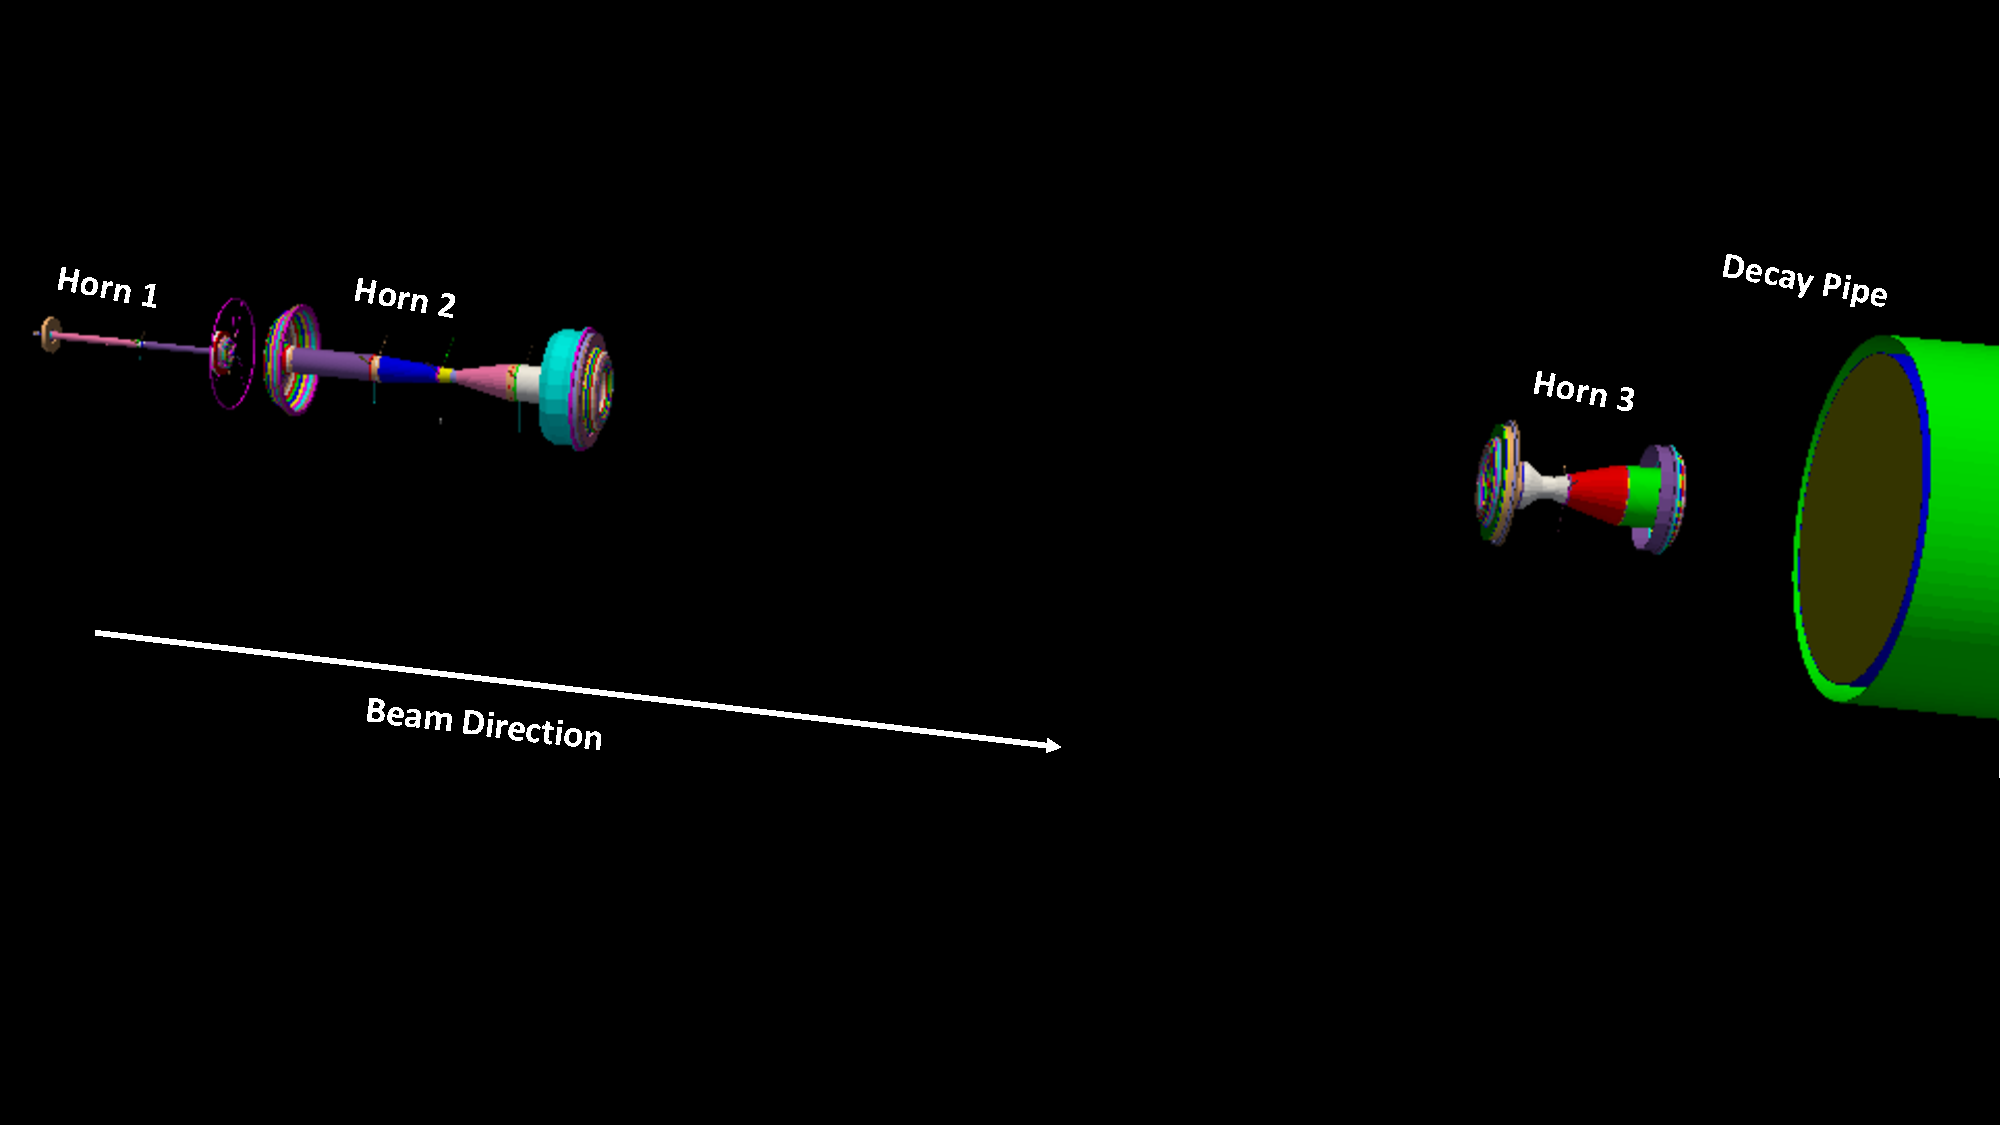
\includegraphics[width=0.7\textwidth]{graphics/Beamline_optimized_sept2017.pdf}\end{dunefigure}


The optimized LBNF neutrino beam design is the result of several years of effort by LBNF and DUNE to identify a focusing system optimized to DUNE's long-baseline physics goals.  This process began with a genetic algorithm that scanned simulations of many different horn and target geometries to identify those that produced the optimal sensitivity to CP violation.  The specific metric used was estimated sensitivity to 75\% of CP phase space after 300 kT MW years of exposure, taking into account the number and neutrino spectra of all neutrino flavors. The resulting beam effectively optimized flux at the first and second oscillation maxima, which also benefits measurements of other oscillation parameters.  The output of the genetic algorithm was a simple design including horn conductor and target shapes.  This design was transformed into a detailed conceptual design by LBNF engineers, and iterated with DUNE physicists to ensure that engineering changes had minimal impact on physics performance.  Relative to the previous NuMI-like design, the optimized design reduces the time to three-sigma coverage of 75\% of CP phase space by 42\%, which is equivalent to increasing the mass of the far detector by 70\%.  It also substantially increases sensitivity to the mass hierarchy and improves projected resolution to quantities such as $\sin^22\theta_{13}$ and $\sin^2\theta_{23}$~\cite{fields_doc_2901}.        

\subsection{On-axis Neutrino Flux and Uncertainties}

\begin{dunefigure}[Neutrino fluxes at the far detector]{fig:flux_flavor}
{Neutrino fluxes at the far detector for neutrino mode (left) and
antineutrino mode (right).  REFERENCE BEAM.  To Be replaced with similar plots for optimized beam. }
    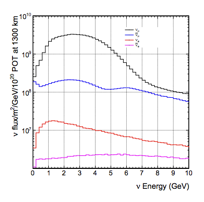
\includegraphics[width=0.45\textwidth]{graphics/Ref_beam_log_flux.png}
     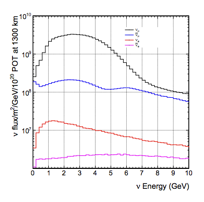
\includegraphics[width=0.45\textwidth]{graphics/Ref_beam_log_flux.png}
\end{dunefigure}


\todo{Add numbers for flavor composition of beam}
Neutrino fluxes for neutrino and antineutrino mode configurations of LBNF are shown in Figure~\ref{fig:flux_flavor}.  In neutrino (antineutrino) mode, the beams are AA\%(BB\%) muon neutrinos (antineutrinos), with wrong-sign contamination making up CC\%(DD\%) and electron neutrino and antineutrino backgrounds EE\%(FF\%).  Although there is also expected to be a small non-zero intrinsic tau neutrino flux, this is not simulated by G4LBNF.  Neutrinos arising from hadron decay at rest are also not simulated.  

\begin{dunefigure}[Flux uncertainties at the far detector as a function of neutrino energy]{fig:flux_uncertainties_flavor}
{Flux uncertainties at the far detector as a function of neutrino energy in neutrino mode (left) and antineutrino mode (right) for, from top to bottom, muon neutrinos, muon antineutrinos, electron neutrinos and electron antineutrinos.   This is for the NDTF optimized flux; it will  be updated with latest beam design.   }
    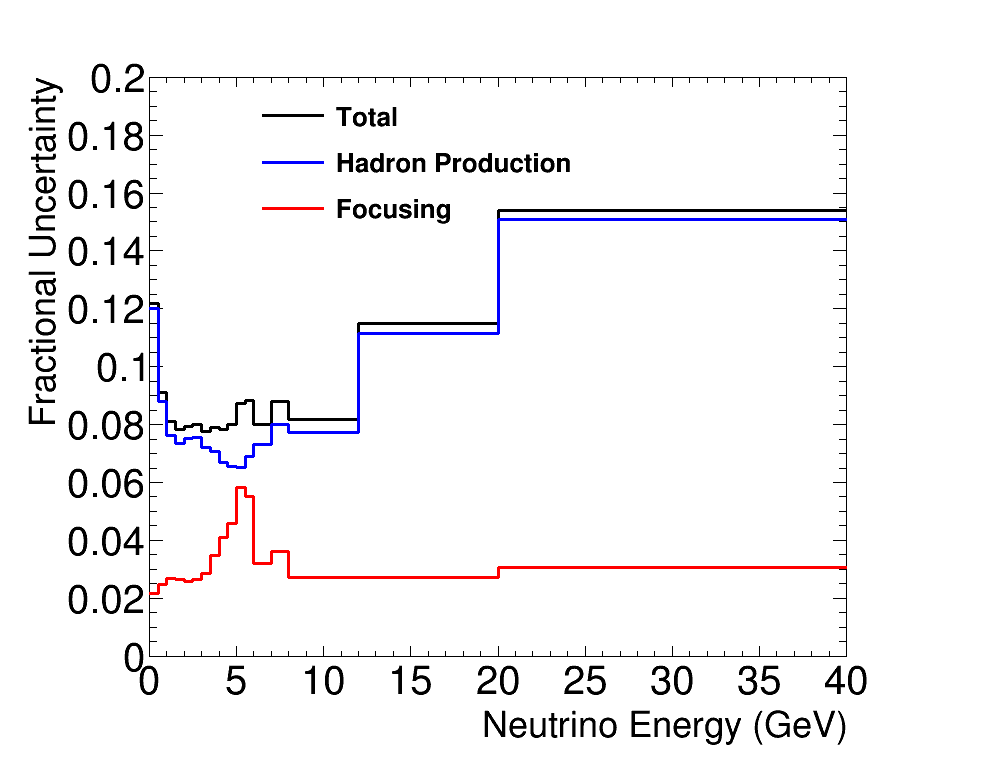
\includegraphics[width=0.4\textwidth]{graphics/error_overlay_numu_neutrino_FD_opt.png}
    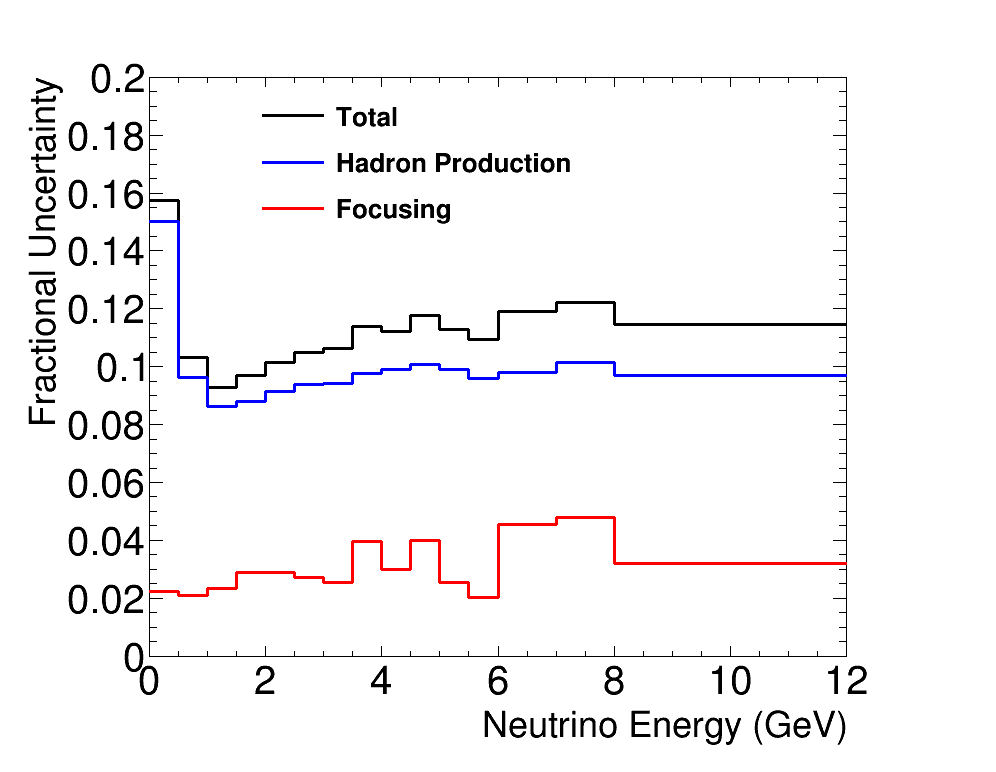
\includegraphics[width=0.4\textwidth]{graphics/error_overlay_numu_antineutrino_FD_opt.png}
    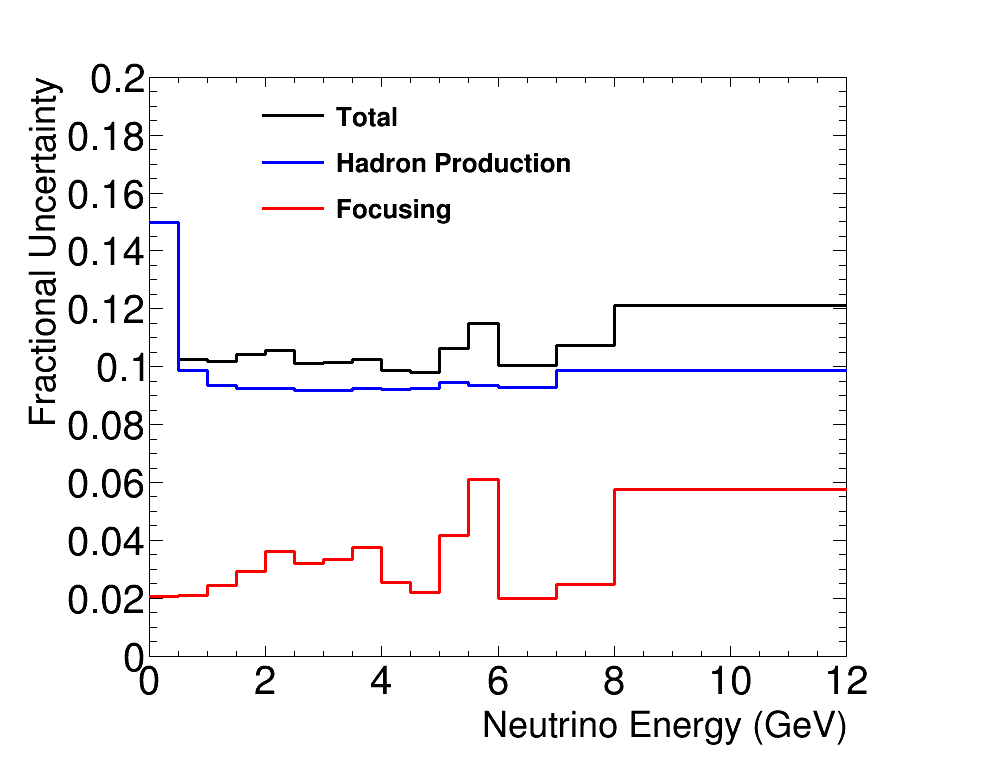
\includegraphics[width=0.4\textwidth]{graphics/error_overlay_numubar_neutrino_FD_opt.png}
    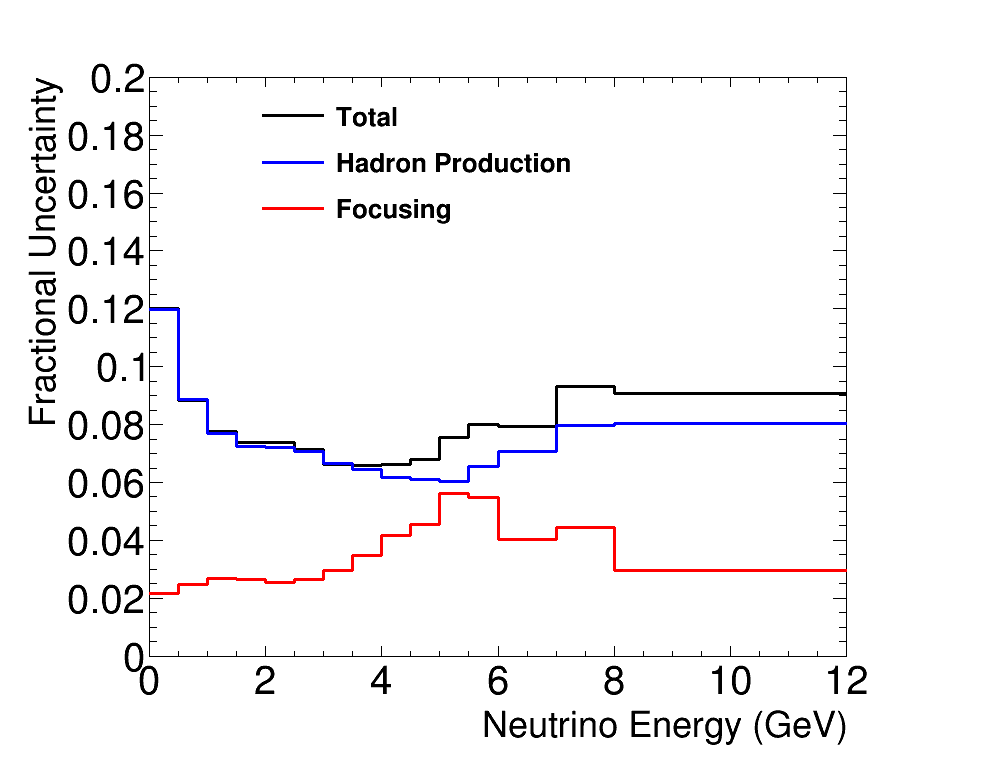
\includegraphics[width=0.4\textwidth]{graphics/error_overlay_numubar_antineutrino_FD_opt.png}
        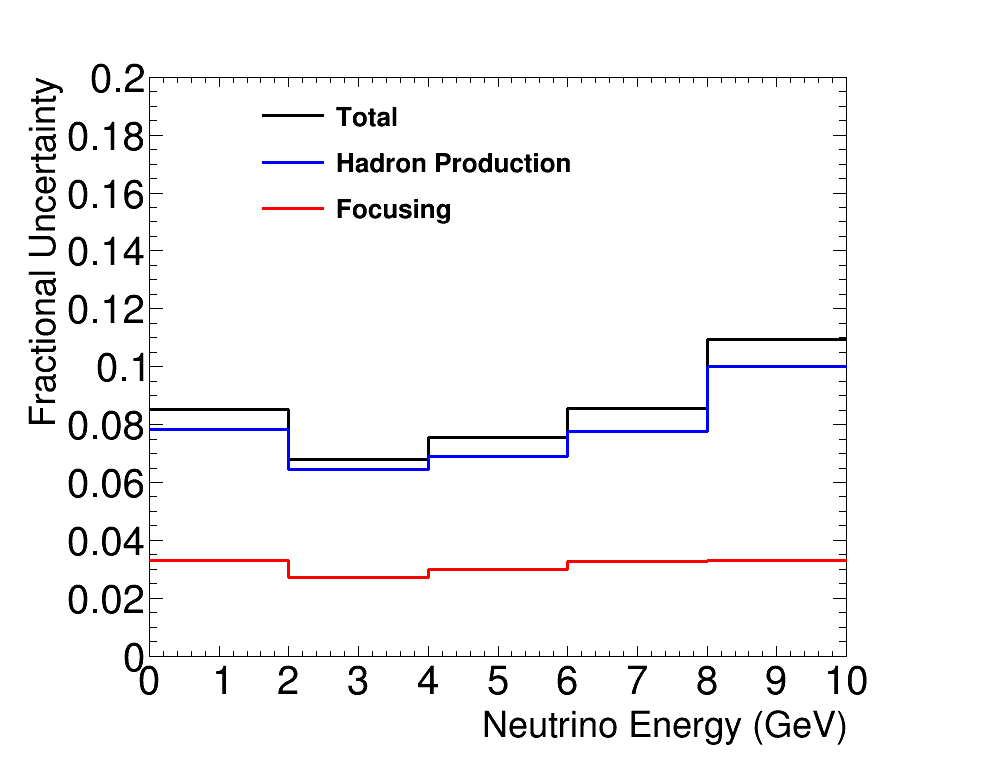
\includegraphics[width=0.4\textwidth]{graphics/error_overlay_nue_neutrino_FD_opt.png}
    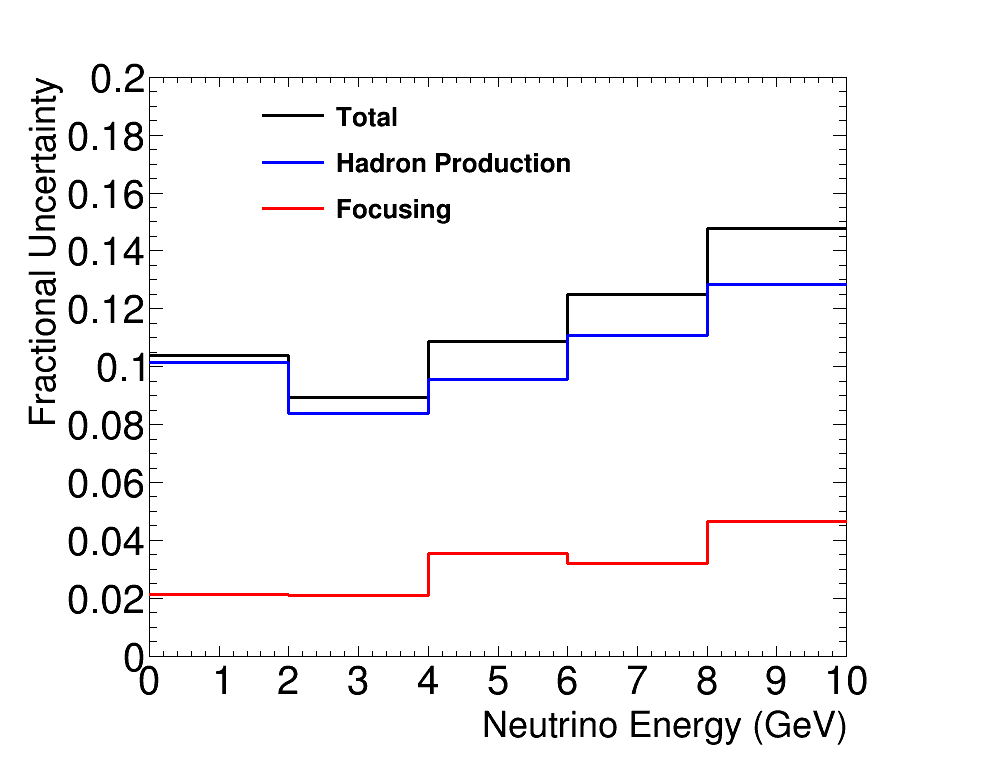
\includegraphics[width=0.4\textwidth]{graphics/error_overlay_nue_antineutrino_FD_opt.png}
        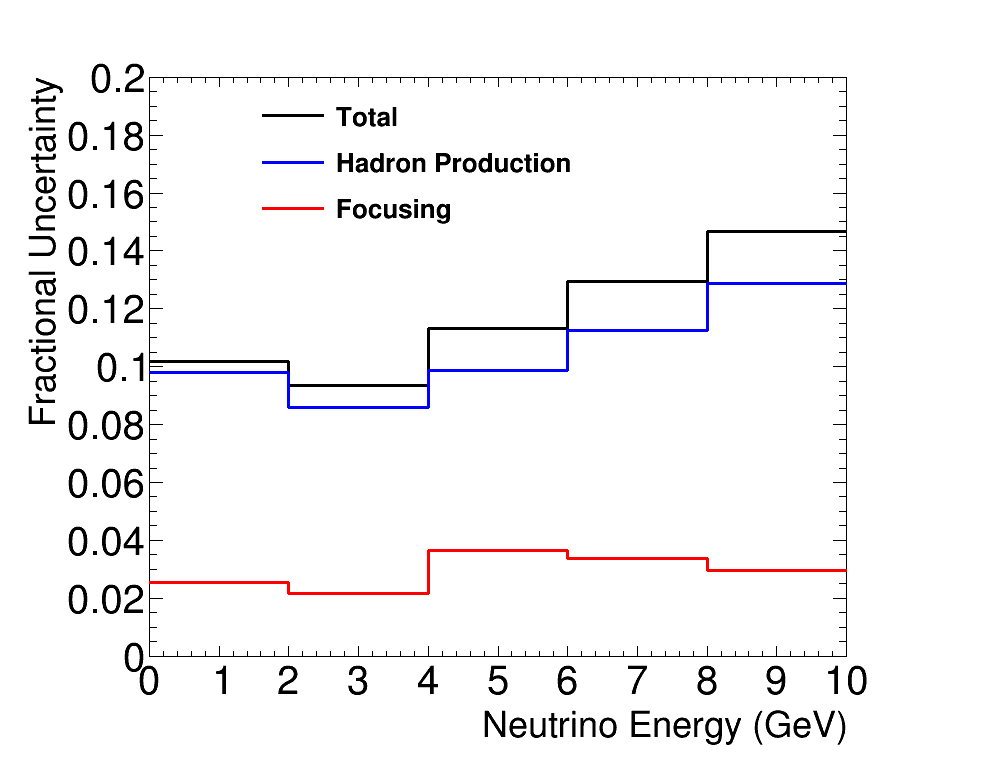
\includegraphics[width=0.4\textwidth]{graphics/error_overlay_nuebar_neutrino_FD_opt.png}
    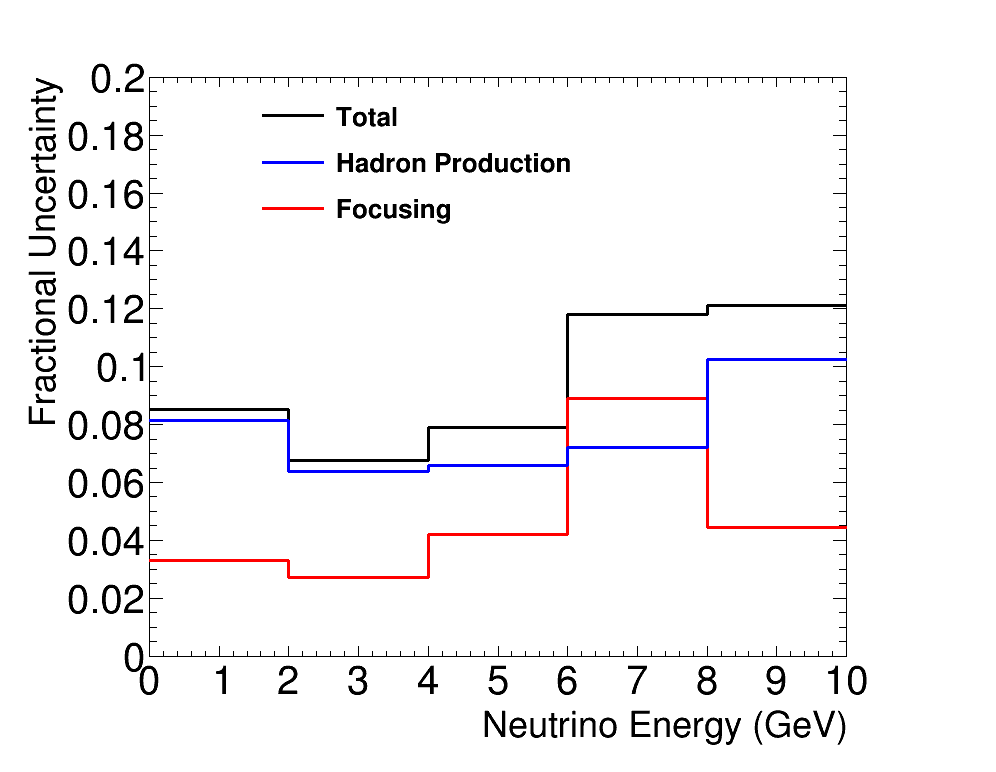
\includegraphics[width=0.4\textwidth]{graphics/error_overlay_nuebar_antineutrino_FD_opt.png}
    \end{dunefigure}




\begin{dunefigure}[Focusing and hadron production uncertainties on the $\nu$ mode $\nu_{\mu}$ flux]{fig:flux_uncertainty_breakdown}
{Focusing (left) and hadron production (right) uncertainties on the neutrino mode muon neutrino flux at the far detector.  This is for an older beam design and will be updated to the latest.  }
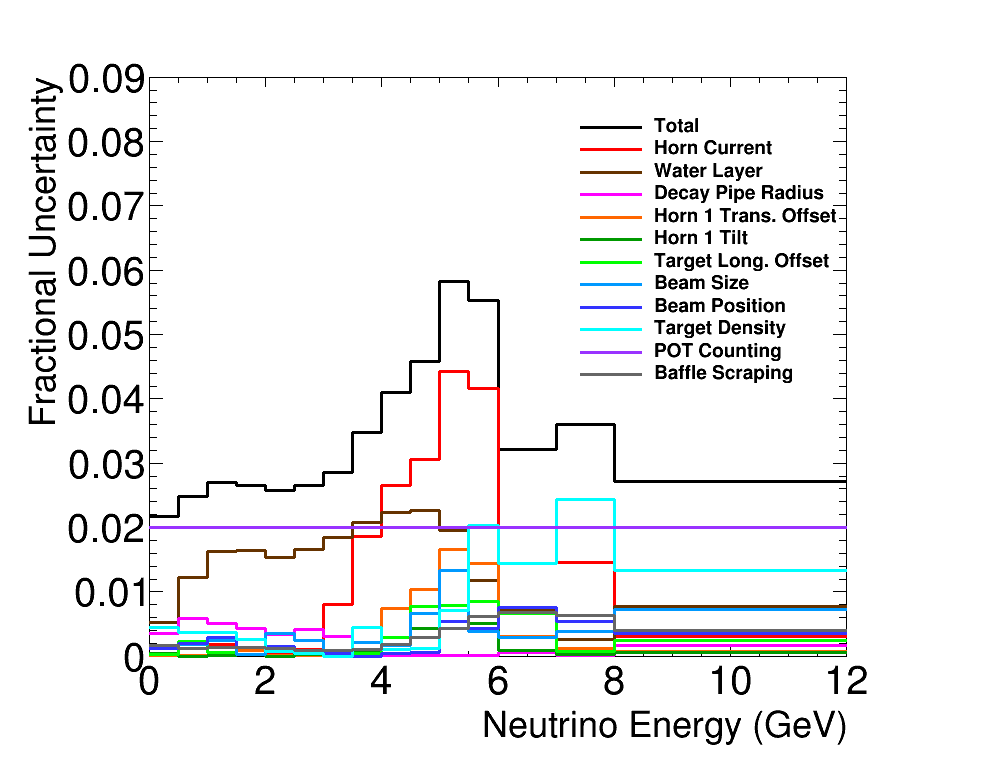
\includegraphics[width=0.45\textwidth]{graphics/focusing_error_overlay_numu_neutrino_FD_opt.png}
    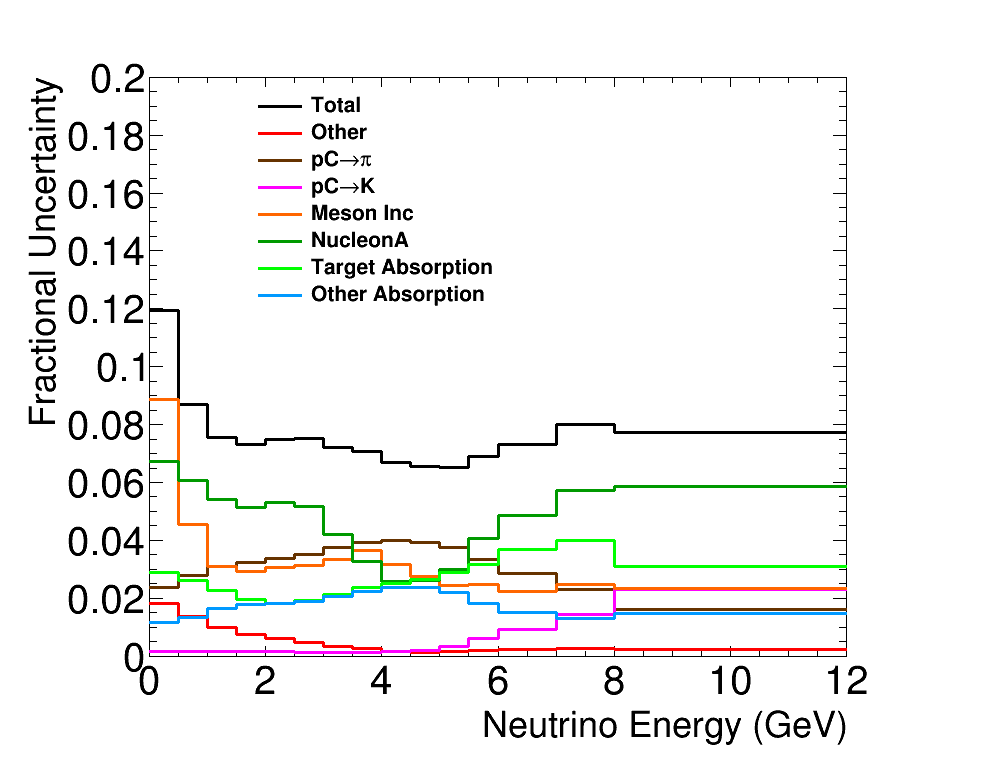
\includegraphics[width=0.45\textwidth]{graphics/HP_error_overlay_numu_neutrino_FD_opt.png}\end{dunefigure}

Uncertainties on the neutrino fluxes arise primarily from uncertainties in hadrons produced off the target and uncertainties in parameters of the beam such as horn currents and horn and target positioning (commonly called "focusing uncertainties").  Uncertainties on the neutrino fluxes arising from both of theses categories of sources are shown in Figure~\ref{fig:flux_uncertainties_flavor}.  Hadron production uncertainties are estimated using the PPFX framework developed by the MINERvA collaboration~\cite{Aliaga:2016oaz, AliagaSoplin:2016shs}, which assigns uncertainties for each hadronic interaction leading to a neutrino in the beam simulation, with uncertainties taken from thin target data (from e.g. the NA49~\cite{NA49} experiment) where available, and large uncertainties assigned to interactions not covered by data.  Focusing uncertainties are assessed by altering beamline parameters in the simulation within their tolerances and observing the resulting change in predicted flux.  An breakdown of the hadron production and focusing into various components are shown in Figure~\ref{fig:flux_uncertainty_breakdown} for the neutrino mode muon neutrino flux at the far detector.    

At most energies, hadron production uncertainties are dominated by the "NucleonA" category, which includes proton and neutron interactions that are not covered by external data.  At low energies, uncertainties due to pion reinteractions (denoted "Meson Inc") dominate.   The largest source of focusing uncertainty is arises from a 1\% uncertainty in the horn current, followed by a 2\% flat uncertainty in the number of protons impinging on the target.   For all neutrino flavors and all neutrino energies, hadron production uncertainties are larger than focusing uncertainties.  However, Hadron production uncertainties are expected to decrease in the next decade, as more thin target data becomes available.  Hadron production measurements taken with a replica target are also being considered and would substantially reduce the uncertainties.  


\begin{dunefigure}[Correlation of flux uncertainties]{fig:flux_uncertainty_correlation}
{Correlation of flux uncertainties.  Each block of neutrino flavor corresponds to bins of energy with bin boundaries of [0.0, 0.5, 1.0, 1.5, 2.0, 2.5, 3.0, 3.5, 4.0, 4.5, 5.0, 5.5, 6.0, 8.0, 10.0, 15.0, 20.0, 40.0, 100.0] for muon neutrinos and antineutrinos and of [0.0, 2.0, 4.0, 6.0, 8.0, 10.0, 20.0, 100.0] for electron neutrinos and antineutrinos. }
    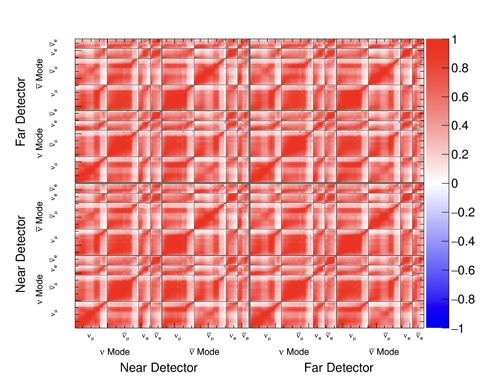
\includegraphics[width=0.9\textwidth]{graphics/correlation_ndtf_opt.png}\end{dunefigure}

Correlations of the total flux uncertainties are shown in Figure~\ref{fig:flux_uncertainty_correlation}.  In general, the uncertainties are highly correlated across energy bins (although the flux in the very high energy tends to be uncorrelated with flux at the peak).  Flux uncertainties are also highly correlated between the near and far detectors and between neutrino mode and antineutrino mode running.  The focusing uncertainties do not affect wrong-sign backgrounds, which reduces correlations between e.g. muon neutrinos and muon antineutrinos in the same running configuration in the energy bins where focusing uncertainties are significant.    

Although the fluxes at the near and far detector are similar, they are not identical.  The ratio of neutrino mode muon neutrino fluxes at the near and far detectors and the uncertainties on the ratio are shown in  Figure~\ref{fig:flux_nearfar}.  The uncertainties are around 1\% or smaller except at the falling edge of the focusing peak, where they rise to 2\% but are still much smaller than the uncertainty on the absolute fluxes.    And unlike the case for absolute fluxes, the uncertainty on the near/far flux ratio is dominated by focusing rather than hadron production uncertainties.  This ratio and its uncertainty are for the fluxes at the center of the detector, and does not take into account small variations in flux across the face of the near detector.     

\begin{dunefigure}[Ratio of neutrino mode muon neutrino fluxes at the near and far detectors]{fig:flux_nearfar}
{Ratio of neutrino mode muon neutrino fluxes at the near and far detectors (left) and uncertainties on the ratio (right) (right).  To be updated. }
    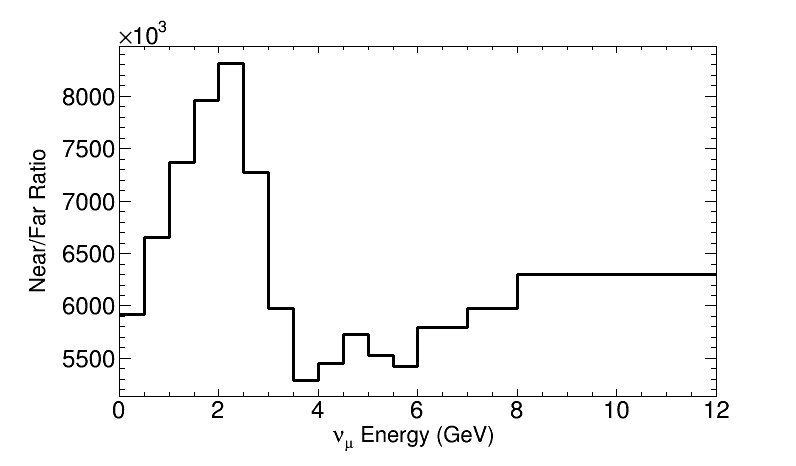
\includegraphics[width=0.45\textwidth]{graphics/nearfar.png}
     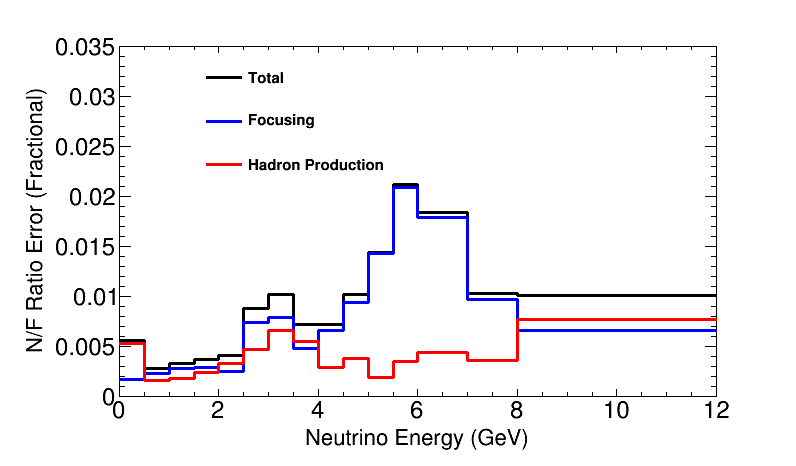
\includegraphics[width=0.45\textwidth]{graphics/nearfarunc.png}
\end{dunefigure}


\subsection{Off-axis Neutrino Flux and Uncertainties}

The neutrino flux spreads beyond the beam directly aimed at the DUNE Far Detector and viable neutrino fluxes extend outward at the near detector hall. The relationship between the parent pion energy and neutrino energy is shown in Fig.~\ref{fig:OAAFluxFigs}; for an ``off-axis'' angle relative to the initial beam direction, the subsequent neutrino energy spectra is narrower and and peaked at a lower energy than the on-axis spectra. At $575\,\textrm{m}$, the location of the near detector hall, a lateral shift of $1\,\textrm{m}$ corresponds to approximately a $0.1^\circ$ change in off-axis angle.

\begin{dunefigure}[optional caption for LoF]{fig:OAAFluxFigs}
{(a) The neutrino energy as a function of parent pion energy for different angles away from the pion momentum vector. Figure from Ref.~\cite{Duffy:2016owt}. (b) The DUNE near detector flux predictions over a range of off-axis positions for a near detector at $575\,\textrm{m}$ downstream of the target station. }
%is subfig package included? I don't think subfloat is working (ZP)
%  \subfloat[C][Off-axis pion decay kinematics]{
    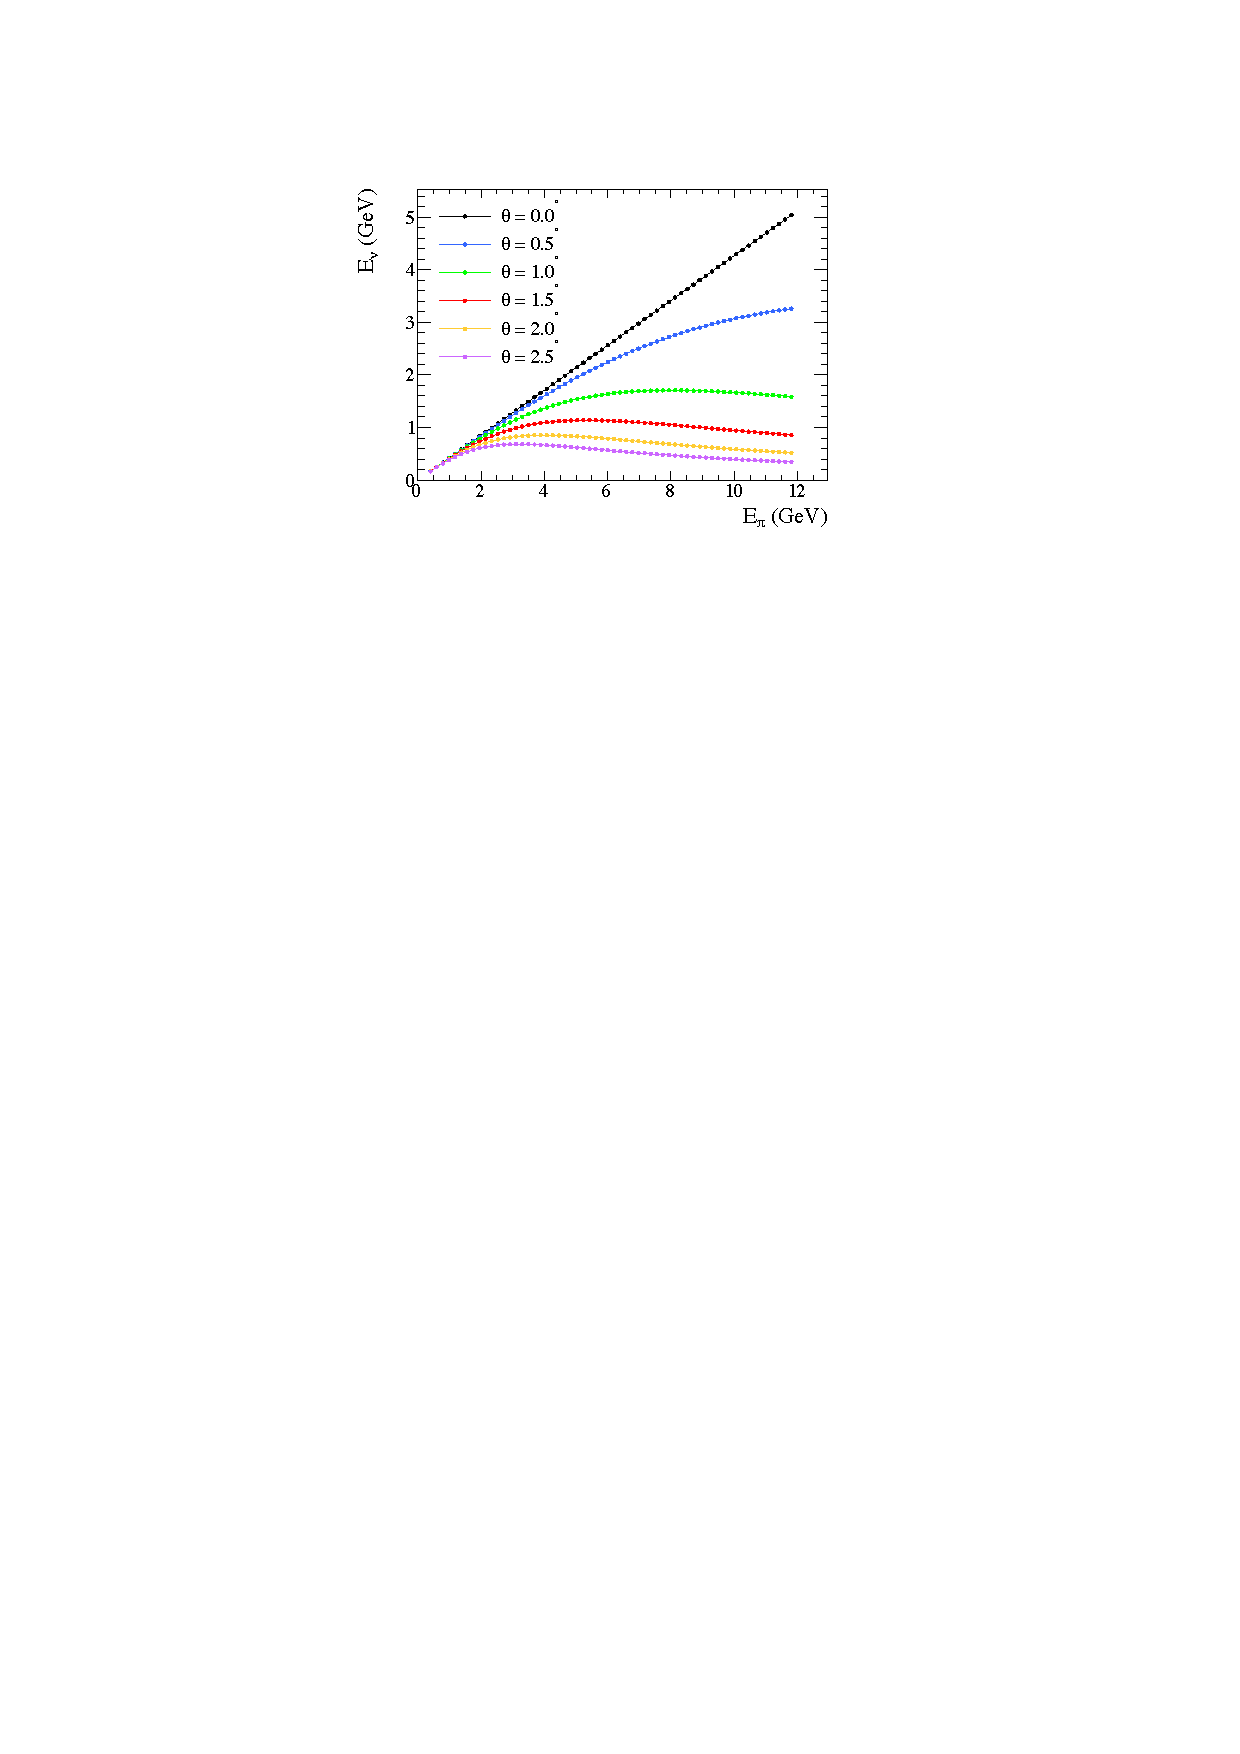
\includegraphics[width=0.4\textwidth]{OATrick}
%    \label{fig:OATrick}
%  }
%  \subfloat[][DUNE near detector flux predictions]{
    \raisebox{0.5em}{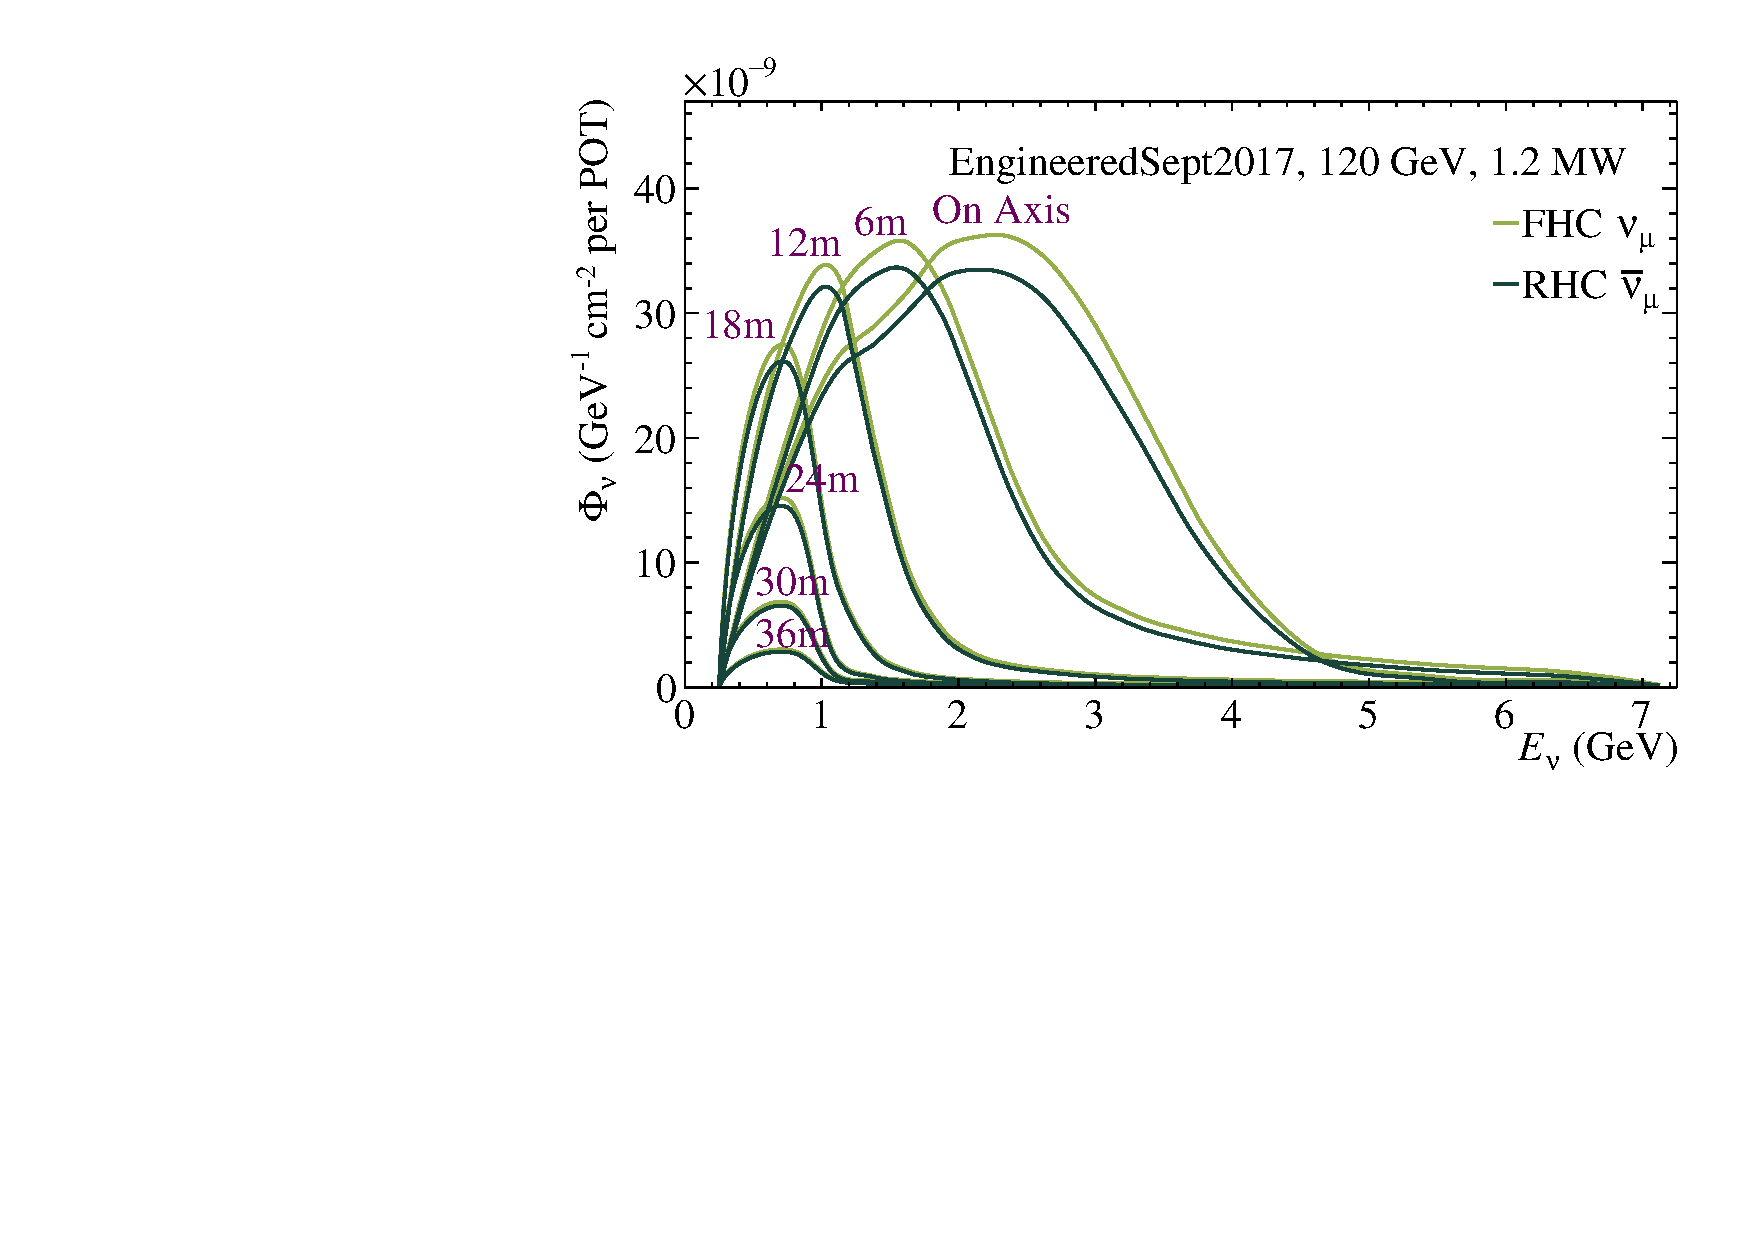
\includegraphics[width=0.40\textwidth]{OffAxisFluxes_1D}}
%    \label{fig:OffAxisFluxes_1D}
%  }
\end{dunefigure}

The intrinsic neutrino flavor-content of the beam varies with off-axis angle. Fig~\ref{OffAxisFluxes_1D_AllSpec} shows the neutrino-mode and anti-neutrino-mode predictions for the four neutrino flavors at the on-axis position, and a moderately off-axis position. At the $30\,\textrm{m}$ position, a second, smaller energy peak at approximately 4 GeV is due to the charged kaon neutrino parents. 
%As both the pion and kaon-parent peaks are significantly narrower in observed neutrino energy at greater off-axis angle, this which may allow for off-axis kaon-parent analyses.

\fixme{Fig~\ref{fig:OffAxisFluxes_1D_AllSpec} is partly redundant with earlier figure, nice if it can be merged? }

\begin{dunefigure}[optional caption for LoF]{fig:OffAxisFluxes_1D_AllSpec}
{The predicted muon neutrino energy spectra at two near detector positions, on axis and $30\,\textrm{m}$ off axis. (a) The predicted neutrino flavor-content of the neutrino-mode (FHC) and anti-neutrino-mode (RHC) beam. (b) The neutrino-mode, muon-flavor predicted flux, separated by the particle that decayed to produce the neutrino. The off-axis spectrum displays a double peak structure due to charged kaon parent decay kinematics. The on-axis kaon-peak occurs at higher neutrino energy and will have a significantly broader energy spread. Top: Beam neutrino flavor content, middle: Beam neutrino flavor content; bottom: Beam neutrino decay-parent species}
    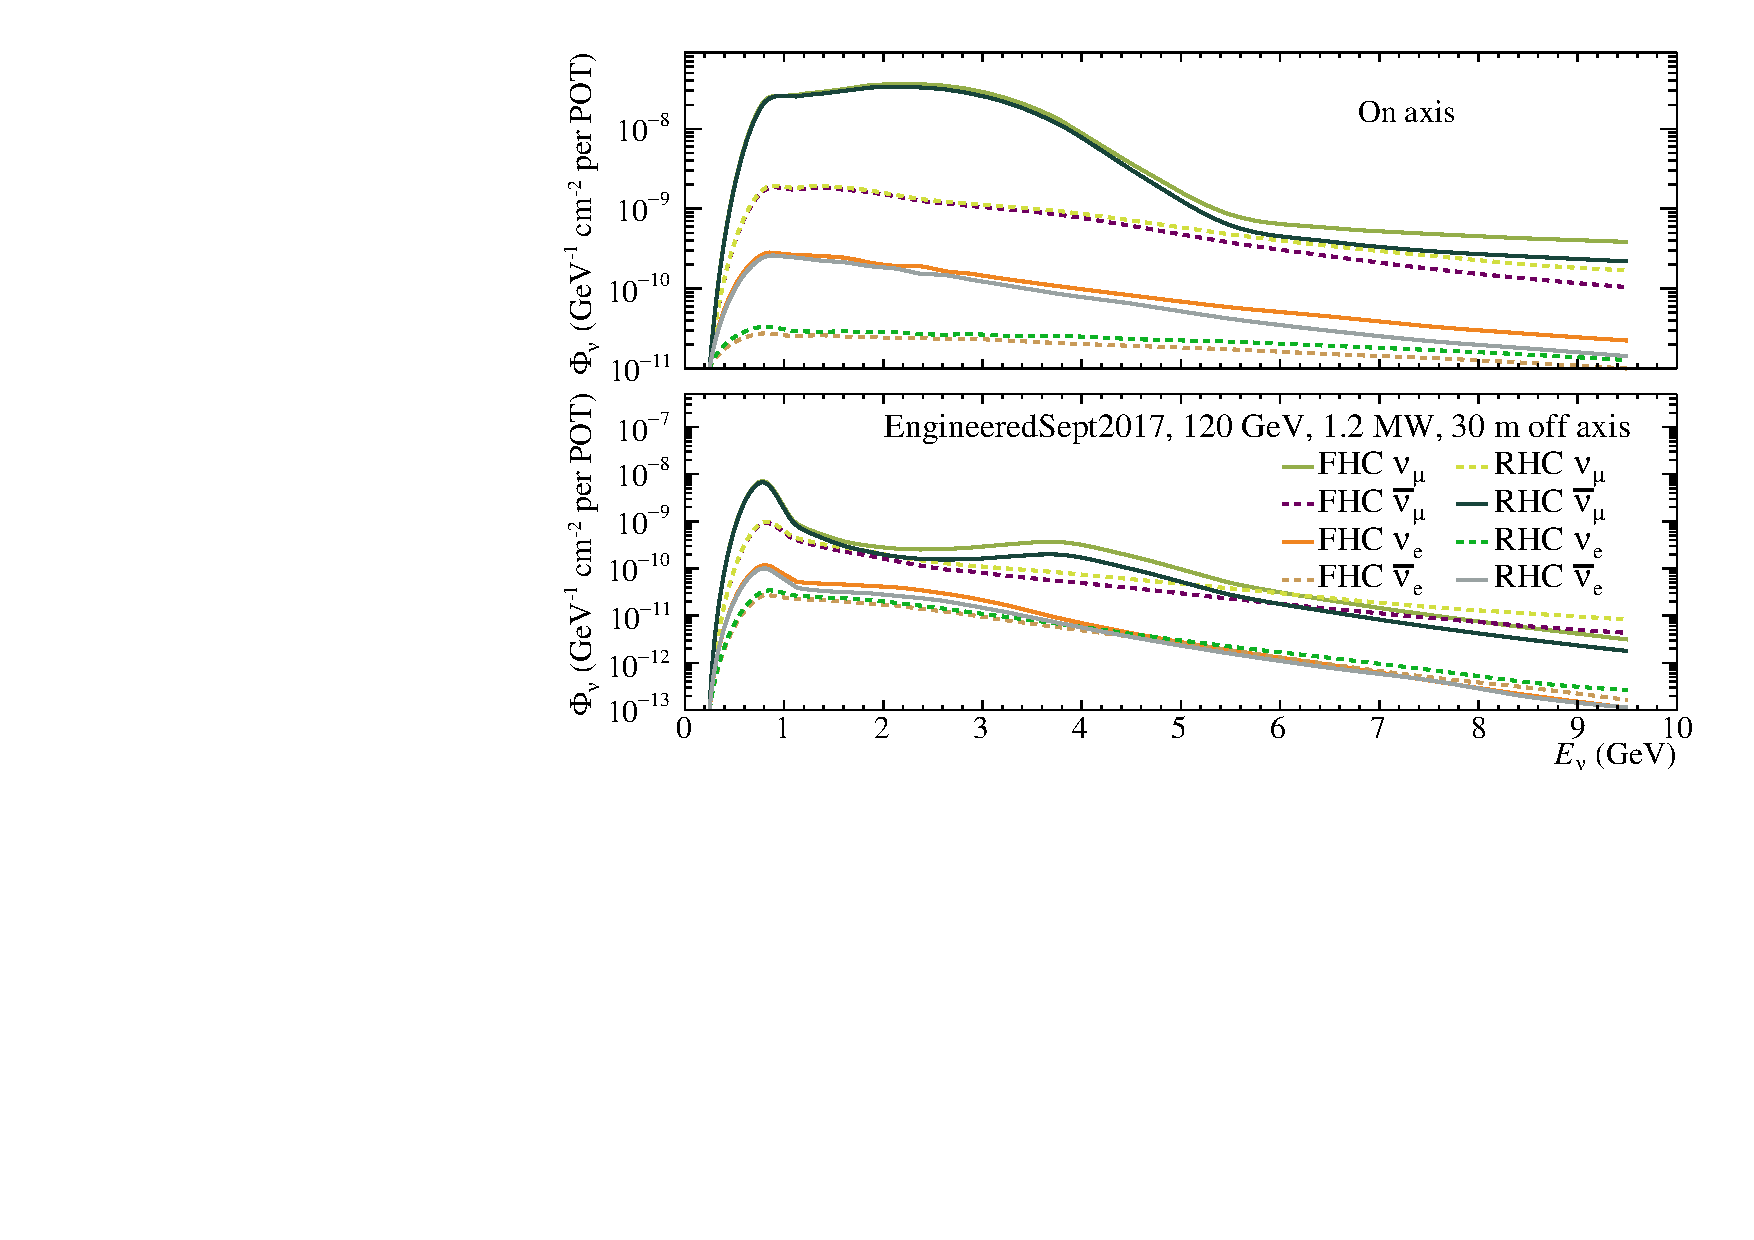
\includegraphics[width=0.8\textwidth]{OffAxisFluxes_1D_AllSpec}
    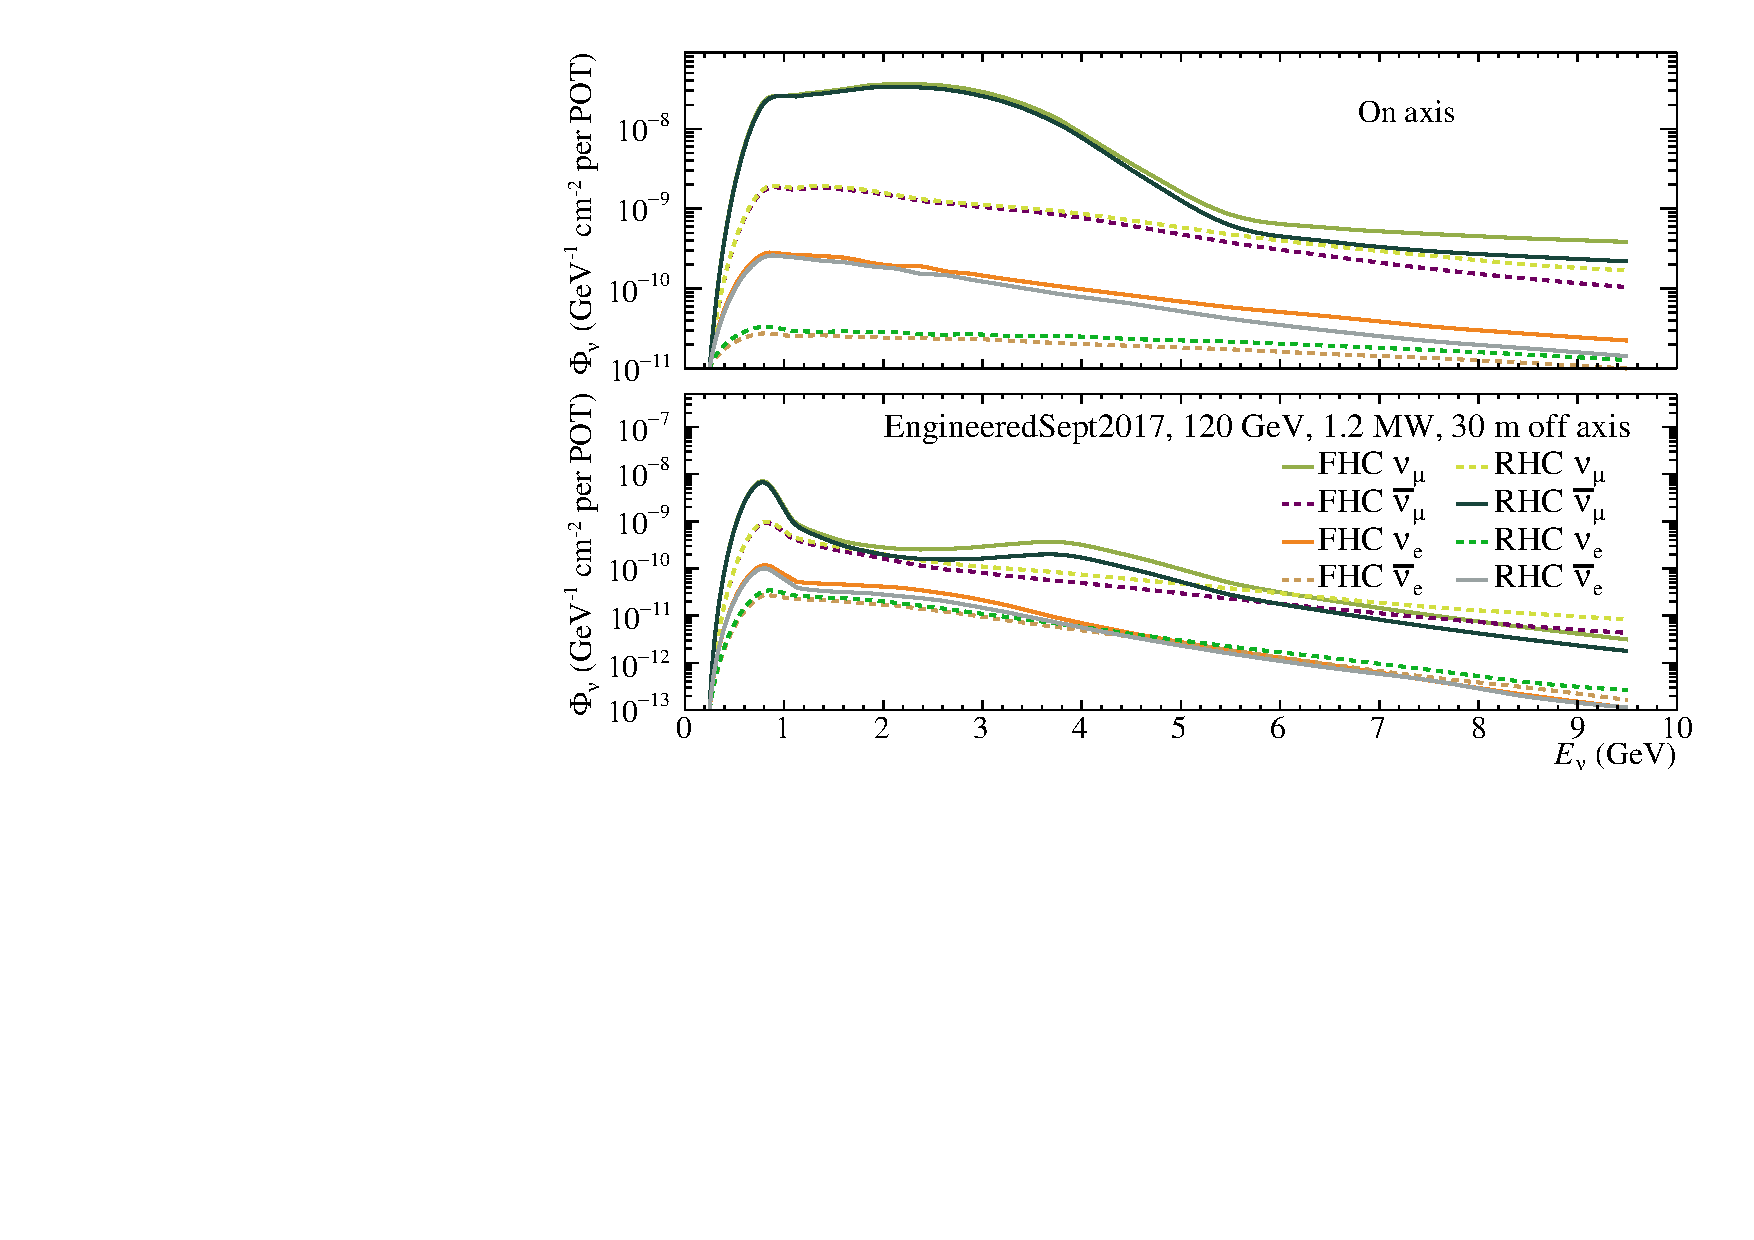
\includegraphics[width=0.8\textwidth]{OffAxisFluxes_1D_AllSpec}
  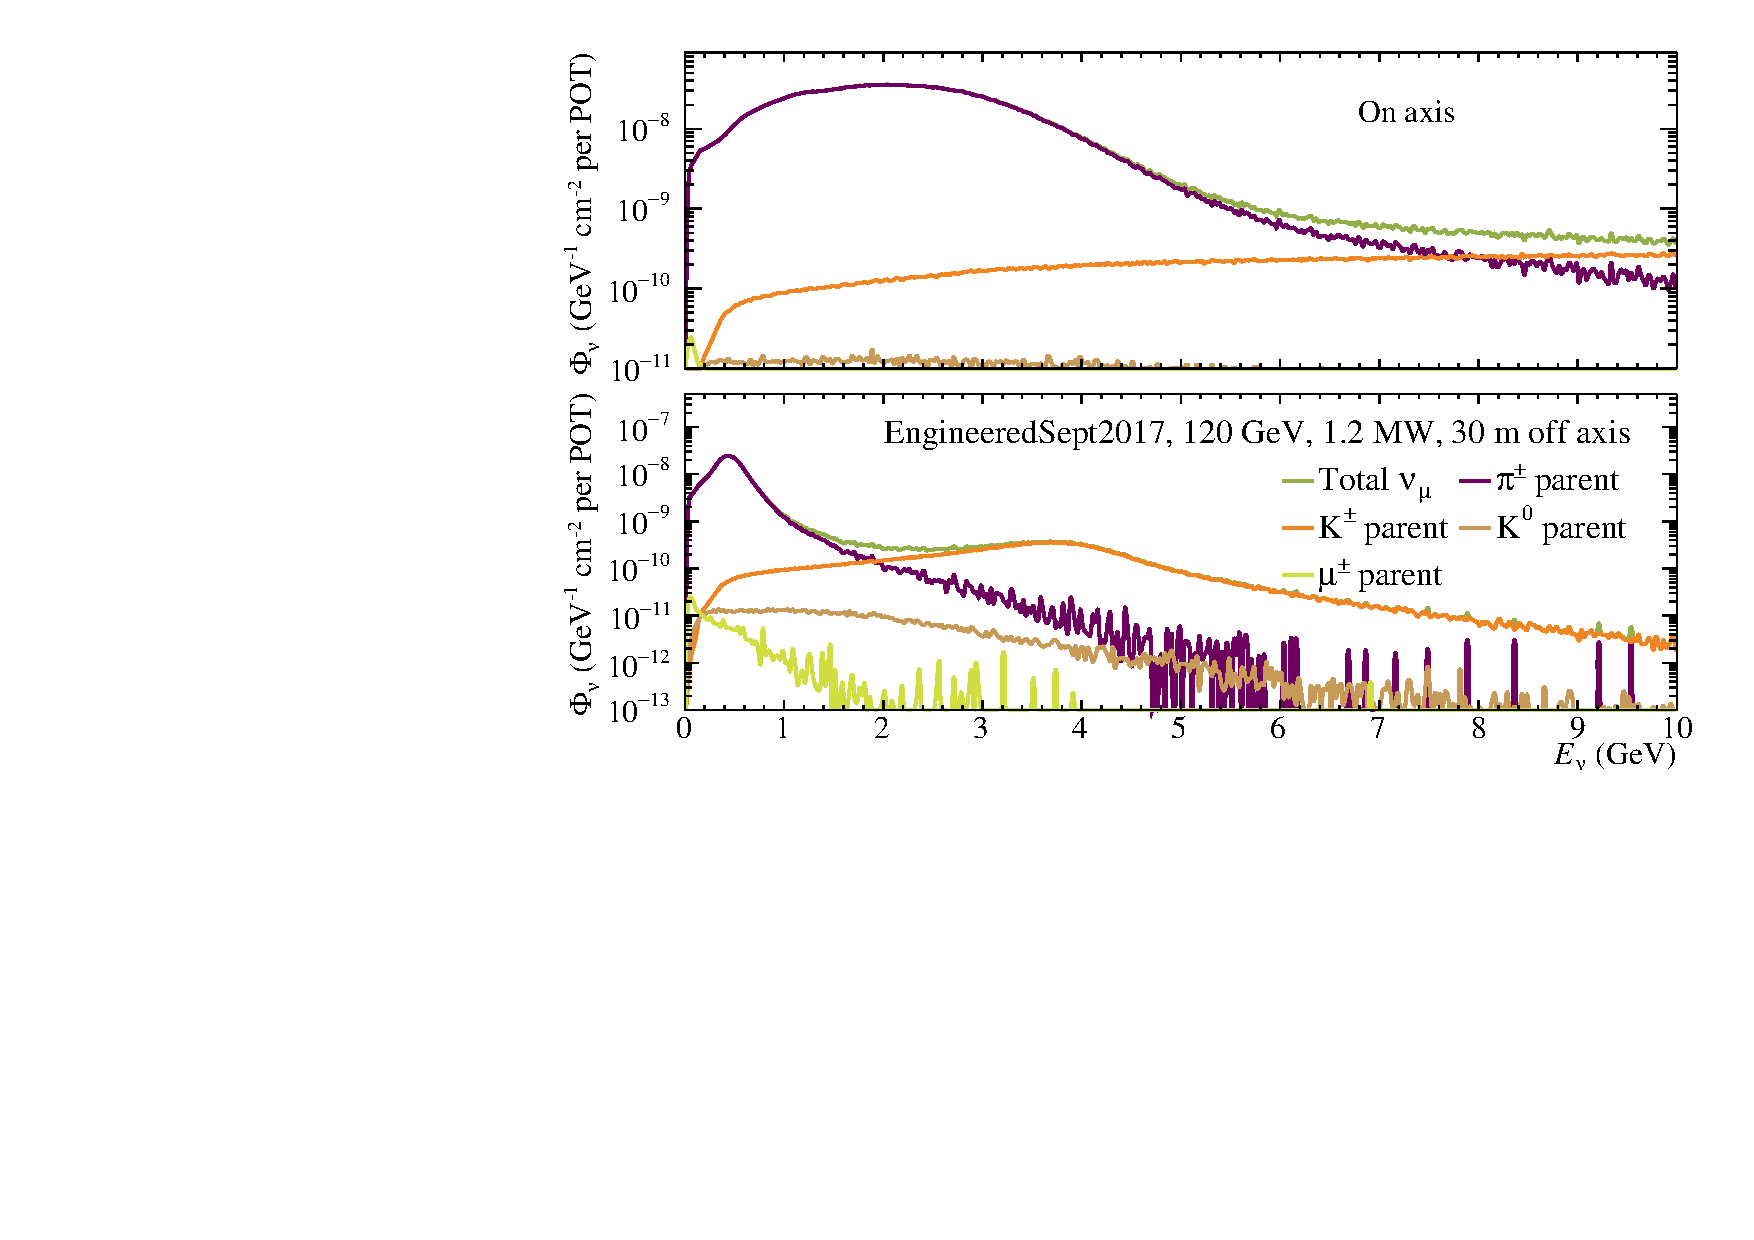
\includegraphics[width=0.8\textwidth]{OffAxisFluxes_1D_Parents}    
    \end{dunefigure}

\fixme{one label per dunefigure; I didn't use label fig:OffAxisFluxes\_1D\_Parents or fig:OAAFluxFigsDetail - may need to fix refs}

The same sources of systematic uncertainty which affect the on-axis spectra also modify the off-axis spectra.  Generally, the size of the off-axis uncertainties is comparable to the on-axis uncertainties and the uncertainties are highly correlated across off-axis and on-axis positions. Studies of extreme changes to horn positions and current indicate that the larger than expected shifts to the horn focusing elements (as has been historically seen in NuMI) would induce significant changes off-axis, and so off-axis flux measurements are useful to diagnose beamline physics.

\fixme{DISCUSS FIGURE: Plot of extreme off-axis angle 1D uncertainty profiles? Can be relative off-axis to on-axis or just off-axis only. }


\subsection{Alternate Beamline Configurations}

Although the LBNF beamline is expected to run for many years in a CP-optimized configuration, it could potentially be modified in the future for other physics goals.  For example, it could be altered to produce a higher energy spectrum in order to measure tau neutrino appearance.  In the standard CP-optimized configuration, about 130 tau neutrino charged current interactions per year are expected at the far detector, before detector efficiency and assuming 1.2 MW beam power.  However, replacing the three CP-optimized horns with two NuMI-like parabolic horns can raise this number to approximately 1000 tau neutrinos per year.  The muon neutrino flux for one such configuration is shown in Figure~\ref{fig:tau-optimized}.  Although the flux in the 0-5 GeV region critical to $\delta_{CP}$ measurements is much smaller, the flux above 5 GeV, where tau neutrino interaction cross section becomes significant, is much larger.  Many other energy distributions are possible by modifying the position of the targets and horns.  Even altering parameters of the CP-optimized horns offers some variablity in energy spectrum, but the parabolic NuMI horns offer more configurability.  Because the LBNF horns are not expected to be remotely movable, such reconfigurations of the beamline would require lengthy downtimes to reconfigure target chase shielding and horn modules.   

\begin{dunefigure}[Comparison of standard and tau-optimized neutrino fluxes]{fig:tau-optimized}
{Comparison of standard and tau-optimized neutrino fluxes.  The tau optimized flux was simulated with a 120 GeV proton beam and two NuMI parabolic horn, with the second horn starting 17.5 downstream from the start of the first horn, and a 1.5 m long, 10 mm wide carbon fin target starting 2m from the upstream face of the first horn.  To be updated.  }
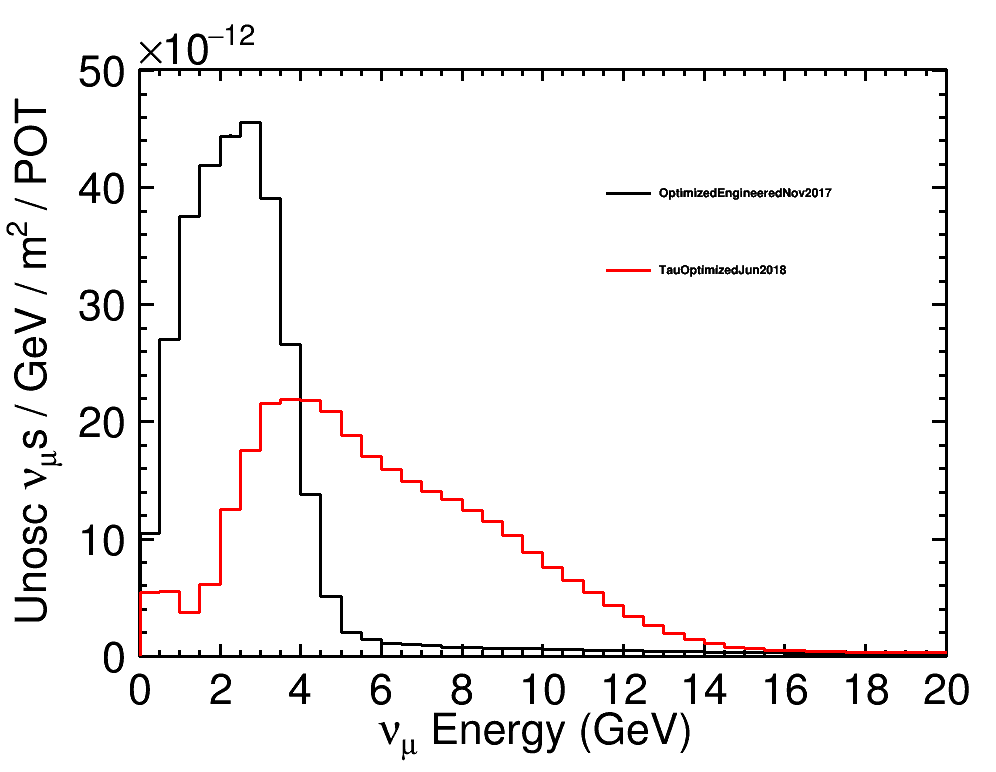
\includegraphics[width=0.7\textwidth]{graphics/tau_optimized.png}
\end{dunefigure}

